\section{Experiments}

In this section, we present our findings from a set of performance experiments that we ran to test the scalability characteristics of Databus. 

\subsection{Experimental setup}

We ran our experiments on two types of machines:

\begin{itemize}
\item Relays and client machines - 12 core 2.56GHz Intel Xeon machines with 48 GB RAM, 1TB SATA RAID 0 and two 1Gbps Ethernet cards
\item Bootstrap servers - 12 core 2.40GHz Intel Xeon machines with 48 GB RAM, 800GB 15K SAS RAID 1+0 and two 1Gbps Ethernet cards.
\end{itemize}

There were three main parameters that we varied:

\begin{itemize}
\item Produce rate - the rate at which events were incoming at the relay buffer
\item Number of consumers - number of services that were consuming events from relays
\item Consumer poll interval - how frequently the consumers were polling the relays for new events
\end{itemize}

For all experiments, we used moderately-sized events with a size of 2.5KB.

The metrics we measured were

\begin{itemize}
\item Throughput - the number of events per second or bytes per second the relay can send out to all consumers or a consumer can read from a relay
\item E2E event latency - the time it takes for an event to propagate from the relay to the consumers
\end{itemize}

\subsection{Relay scalability}

Figure \ref{fig:relay_throughput} shows the first set of experiments where we measured the maximum outbound throughput that a relay can support to clients. We used a relay with an already pre-filled buffer and measured the maximum speed at which multiple clients can read from the relay. We also varied the frequency at which consumers poll the relay. The latter parameter allowed us to test what is the impact of pulling less frequent but bigger batches of events. We expected that less frequent but bigger batches will allow the relay to support larger number of consumers.

\begin{figure}
\centering
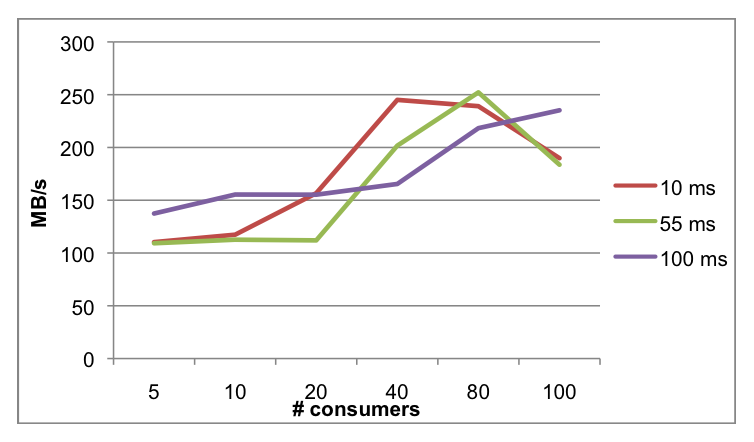
\epsfig{file=figures/relay_throughput.eps, width=3in}
\caption{Relay throughput scalability depending on poll interval}
\label{fig:relay_throughput}
\end{figure}

The experiments confirmed our hypothesis. With lower latency and fast consumers (as the ones that we used for our experiments), we can quickly saturate the network bandwindth. Once we go over a certain number of clients, we actually see performance degradation due to increased number of context switches.Larger poll intervals allow the relay to support larger number of clients without performance degradation.

The second set of experiments on Figure \ref{fig:latency-poll10} aimed at testing how writes to the relay buffer affected relay scalability. For this set of experiments, we gradually increased the update rate at the data source and measured the throughput and latency at the clients. Our goal was to detect when bottlenecks on the relay cause the clients to fall behind the stream of updates from the data sources. Further, at the higher update rates, we also tested how server-side filtering affects scalability.

We fixed the consumer poll interval at 10ms.Therefore, the consumers can expect on average 5 ms latency due to the poll frequency.   

\begin{figure}
\centering
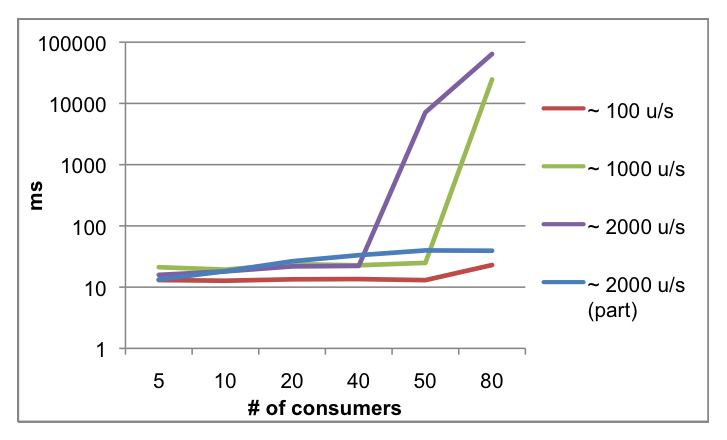
\epsfig{file=figures/e2e_latency.eps, width=3in}
\caption{Latency to consumers}
\label{fig:latency-poll10}
\end{figure}

What the results of the above experiment showed was that overall the Databus overhead was 6-15ms depending on the update rate. For 100 update/s, the relay showed slightly increased latency at around 80 consumers and shot up at around 100 consumers when we hit the outbound network limit. We saw a similar pattern at higher update rates where we hit that bottleneck earlier. As expected, adding server-side filtering improved significantly the maximum number of supported clients and we ran out of test machines before we could hit the max number of clients. The additional relay-side processing increased the CPU utilization which led to an increased in the latency by about 5-10ms.

The above conclusions were confirmed on Figure \ref{fig:throughput-poll10} by the measurements of the rate at which the consumers were recieving the events. Up to the afore-mentioned thresholds, the event rate at the consumers was keeping up with the produce rate. Beyond the thresholds, the maximum throughput at the client drops noticeably.


\begin{figure}
\centering
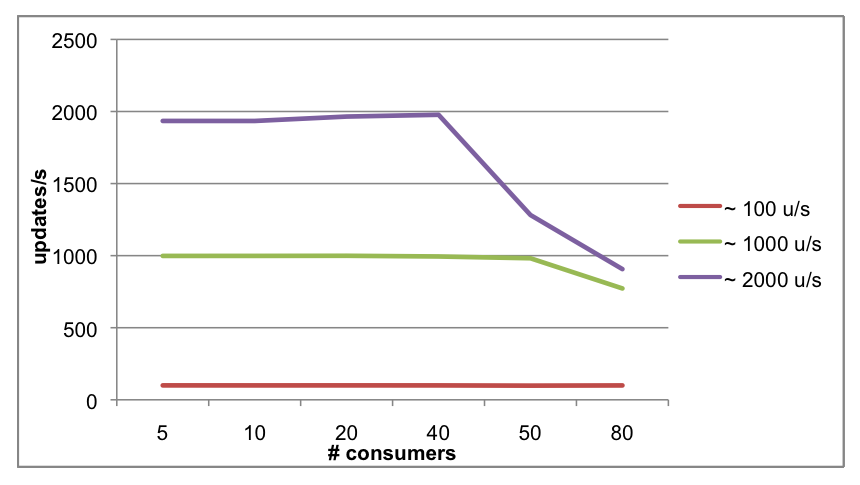
\epsfig{file=figures/consumer_throughput.eps, width=3in}
\caption{Throughput at consumers when varying update rate}
\label{fig:throughput-poll10}
\end{figure}


\subsection{Bootstrap scalability}

For our bootstrap performance experiments, we focused on the interesting and novel aspect of the bootstrap server: the ability to serve compressed deltas of events instead of replaying all updates. 

For this experiment, we introduced a new parameter: the ratio between updates to existing keys (including deletes) versus the total number of change records. This parameter models the benefit of returning only the latest version of the value for a given key. The goal of the experiment is to find the point at which the cost of finding the smaller number of changes in delta which have potentially worse layout on disk meets the cost of the sequential scan over the larger-sized log store. 

\begin{figure}
\centering
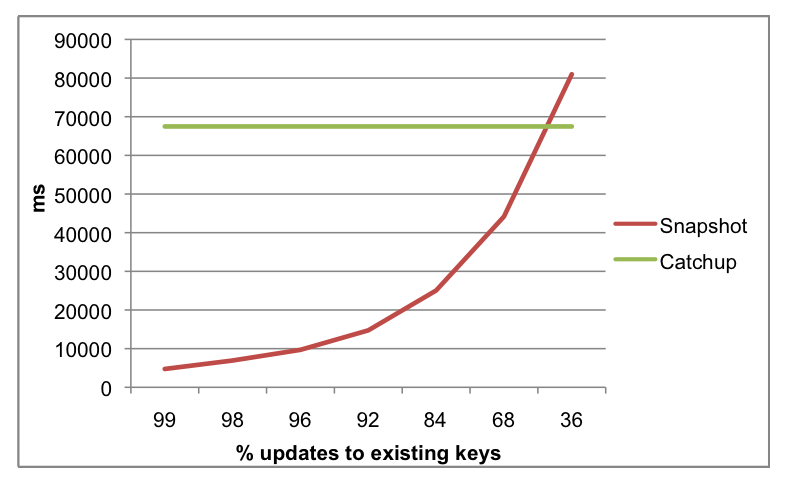
\epsfig{file=figures/snapshot_vs_catchup.eps, width=3in}
\caption{Time to bootstrap 1 hour of changes using a Snapshot delta or Catch-up log}
\label{fig:snapshot_vs_catchup}
\end{figure}

What our experiments showed that with maintaining the appropriate index structures on the snapshot store, returning compressed deltas from the snapshot store is very efficient. The break-even point is when about half of the change records contain updates to existing keys. This case covers a surprisingly large number of the data change patterns at LinkedIn. 


